\pagebreak
\section{Steering test - Linear area for \si{K_p}} \label{app:LinearAreaKp}
\textbf{Name: Group 510}\\
\textbf{Date: 30/09 - 2015}

\subsubsection{Purpose}


\subsubsection{Setup}


\subsubsection{List of Equipment}

\begin{table}[H]
\begin{tabular}{|l|l|p{4cm}|}
\hline%------------------------------------------------------------------------------------
  \textbf{Instrument}                        &  \textbf{AAU-no.}  &  \textbf{Type}       \\
\hline%------------------------------------------------------------------------------------
  Oscilloscope                               &  64672             &  Agilent DSO6034A    \\
\hline
\end{tabular}
\end{table}

\subsubsection{Procedure}

\begin{enumerate}
  \item S
  \item S
  \item S
  \item S
  \item S
  \item S
\end{enumerate}

\subsubsection{Results}

\begin{flalign}
  \eq{\tau_{mec}}{0,238} \tx{ s}&&\nonumber
\end{flalign}

\begin{figure}[H]
  \centering
 	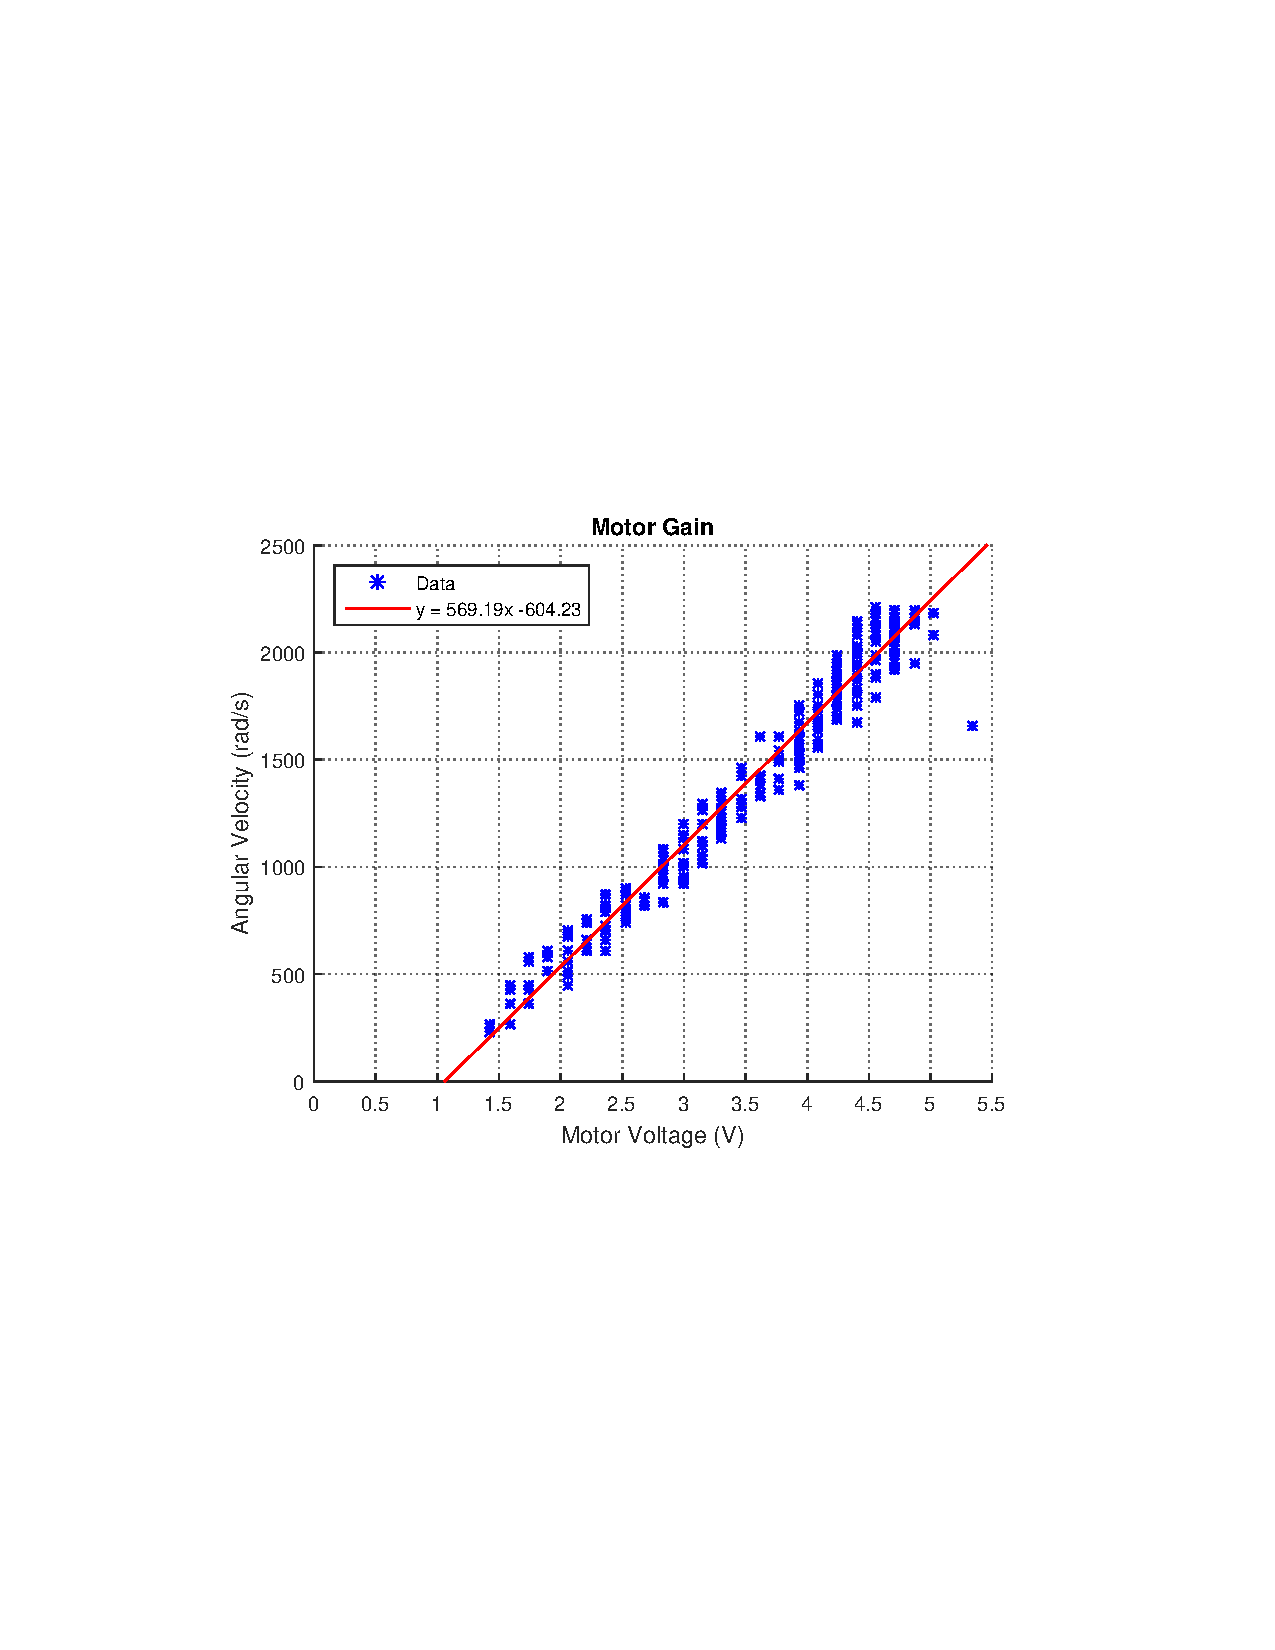
\includegraphics[width=.8\textwidth]{figures/motorGain.pdf}
  \caption{A plot of the motor's step response, where the input is motor voltage and the output is the angular velocity. The blue dots indicates the measurements and the red line is the tendency line.}
	\label{motorGain}
\end{figure}
%
